% =====================================================================
%  EC527 Final Project. Multi-tier Temporally Blocked SOR
%  Compile: pdflatex report.tex (twice for cross-references)
% =====================================================================
\documentclass[11pt]{article}

\usepackage[a4paper,margin=1in]{geometry}
\usepackage{graphicx}
\usepackage{amsmath, amssymb}
\usepackage{booktabs}
\usepackage{xcolor}
\usepackage{hyperref}
\hypersetup{colorlinks=true,linkcolor=black,urlcolor=blue,citecolor=black}
\usepackage{listings}
\usepackage{caption}
\usepackage{subcaption}
\usepackage{enumitem}

\lstset{
    basicstyle=\ttfamily\small,
    keywordstyle=\bfseries,
    commentstyle=\itshape\color{gray!70!black},
    breaklines=true,
    columns=fullflexible,
    showstringspaces=false,
    frame=tb,
    framerule=0.4pt,
    aboveskip=0.6em,
    belowskip=0.6em,
}

\graphicspath{{report_images/}}

\title{\vspace{-3em}Structured-Grid SOR with Temporal Blocking:\\[0.2em]
        \large from one Xeon thread to a CUDA-tiled L40S}
\author{Che-Yu Yu \\ EC527, Spring 2026}
\date{\today}

\begin{document}
\maketitle

% =====================================================================
\section{Description of the Algorithm}
% =====================================================================

\subsection{Mathematical foundation}

We solve the 2D Laplace equation on the unit square with Dirichlet
boundary data:
\begin{equation}
\nabla^2 u(x,y) = 0,\qquad u\big|_{\partial\Omega} = g(x,y).
\label{eq:laplace}
\end{equation}
On a uniform $N{\times}N$ grid with spacing $h{=}1/(N{-}1)$, the
second-order centred difference rearranges to the canonical 5-point
stencil shown in Figure~\ref{fig:stencil}:
\begin{equation}
u_{i,j} = \tfrac{1}{4}\!\left(u_{i-1,j} + u_{i+1,j}
                + u_{i,j-1} + u_{i,j+1}\right).
\label{eq:5point}
\end{equation}

\begin{figure}[h!]
\centering
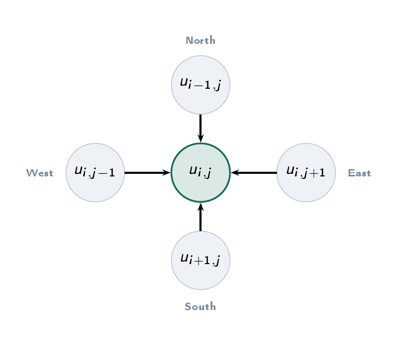
\includegraphics[width=0.42\linewidth]{5points.png}
\caption{The 5-point Laplacian stencil. Each interior cell averages
its four orthogonal neighbours.}
\label{fig:stencil}
\end{figure}

Equation~\eqref{eq:5point} is the Jacobi update. Successive
Over-Relaxation (SOR) adds a relaxation parameter $\omega$ to the
Gauss-Seidel update:
\begin{equation}
u_{i,j}^{(k+1)} = (1-\omega)\,u_{i,j}^{(k)}
+ \frac{\omega}{4}\!\left(u_{i-1,j}^{(k+1)}
                       + u_{i+1,j}^{(k)}
                       + u_{i,j-1}^{(k+1)}
                       + u_{i,j+1}^{(k)}\right).
\label{eq:sor}
\end{equation}
The right-hand side mixes already-updated and not-yet-updated
neighbours. For the Poisson problem on a uniform grid, the optimal
relaxation parameter is
\begin{equation}
\omega_{\text{opt}} = \frac{2}{1 + \sin\!\bigl(\pi/(N{-}1)\bigr)}
\;\approx\; 2 - \frac{2\pi}{N}.
\label{eq:omega-opt}
\end{equation}
That gives $O(N)$ iterations for tuned SOR vs $O(N^2)$ for Jacobi.
We verify this experimentally in §\ref{sec:omega}.

\subsection{The specific algorithmic form used}

We implemented three forms of the sweep. The \emph{baseline} is a
straight scan-order rewrite of \eqref{eq:sor}:

\begin{lstlisting}[language=C]
/* baseline SOR, scan order, in-place: sequential */
for (i = 1; i < N-1; i++)
  for (j = 1; j < N-1; j++) {
    sum = u[i-1][j] + u[i+1][j] + u[i][j-1] + u[i][j+1];
    u[i][j] = (1.0f - OMEGA) * u[i][j] + (OMEGA * 0.25f) * sum;
  }
\end{lstlisting}

\noindent The loop-carried dependency forbids parallelising the outer
loop directly. Two ways out:

\paragraph{Red-black SOR.} Colour the grid like a checkerboard. Red
cells depend only on black cells, so each colour can be updated in
parallel:

\begin{lstlisting}[language=C]
for (parity = 0; parity < 2; parity++) {
  #pragma omp parallel for
  for (i = 1; i < N-1; i++) {
    int j0 = ((i + parity) & 1) ? 1 : 2;
    for (j = j0; j < N-1; j += 2) {
      sum = u[i-1][j] + u[i+1][j] + u[i][j-1] + u[i][j+1];
      u[i][j] = (1.0f - OMEGA) * u[i][j] + (OMEGA * 0.25f) * sum;
    }
  }
}
\end{lstlisting}

\noindent Used in \texttt{sor2d\_rb.c} for the omega-tuning study
(§\ref{sec:omega}, E08).

\paragraph{Jacobi ping-pong.} Read from \texttt{src}, write to
\texttt{dst}, swap. No within-sweep dependency:

\begin{lstlisting}[language=C]
#pragma omp parallel for
for (i = 1; i < N-1; i++)
  for (j = 1; j < N-1; j++) {
    nb = 0.25f * (src[i-1][j] + src[i+1][j] + src[i][j-1] + src[i][j+1]);
    dst[i][j] = src[i][j] - OMEGA * (src[i][j] - nb);
  }
swap(&src, &dst);
\end{lstlisting}

\noindent We trade convergence rate (stable only for
$\omega \in (0, 1]$ on large grids; we use $\omega{=}0.9$) for clean
parallelism and the ability to do temporal blocking.

\paragraph{Temporal blocking (the shrinking trapezoid).} For each
super-step of $T$ Jacobi sweeps:
\begin{enumerate}[leftmargin=1.4em,itemsep=2pt,topsep=2pt]
  \item Tile the grid into $B{\times}B$ output regions
        (Figure~\ref{fig:spatial-blocking}).
  \item For each tile, load a $(B{+}2T)^2$ scratch buffer.
  \item Run $T$ in-scratch Jacobi sweeps; the valid region shrinks by
        one cell per side per sub-step
        (Figure~\ref{fig:halo-time}).
  \item Write the central $B^2$ back to \texttt{dst}.
\end{enumerate}
DRAM traffic for the central cells drops by a factor of $T$. The cost
is redundant halo work: the work multiplier is $((B{+}2T)/B)^2$. We
measure its unimodal optimum in §\ref{sec:cpu-results} (E04).

\begin{figure}[h!]
\centering
\begin{subfigure}[b]{0.49\linewidth}
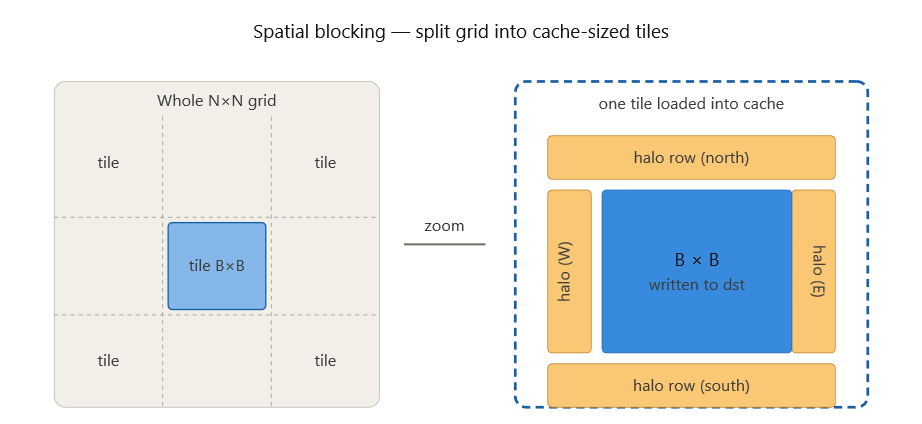
\includegraphics[width=\linewidth]{spatial_blocking.png}
\caption{Spatial blocking: per-thread $B{\times}B$ tiles with a
1-cell halo.}
\end{subfigure}\hfill
\begin{subfigure}[b]{0.49\linewidth}
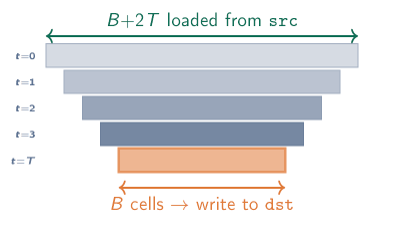
\includegraphics[width=\linewidth]{HALO_time.png}
\caption{Temporal blocking: load $B{+}2T$ cells, do $T$ sub-steps;
the valid region shrinks by one cell per side per sub-step.}
\end{subfigure}
\caption{Spatial vs temporal blocking.}
\label{fig:spatial-blocking}
\label{fig:halo-time}
\end{figure}

Variable glossary:
\begin{itemize}[leftmargin=1.4em,itemsep=1pt,topsep=1pt]
  \item $N$. Grid side; interior is $(N{-}2)^2$ cells.
  \item $B$. Spatial block size.
  \item $T$. Temporal halo (sub-sweeps fused per DRAM round-trip).
  \item $\omega$. Relaxation factor. $0.9$ for ping-pong kernels;
        $\omega_{\text{opt}}{\approx}2{-}2\pi/N$ for red-black.
  \item iters. Total sweep count; must satisfy
        \texttt{iters \% T == 0} for temporal kernels.
  \item TOL. Convergence tolerance ($10^{-5}$).
\end{itemize}

\subsection{Implementation reality check}
\label{sec:reality-check}

\paragraph{Two paths to parallelism.} Scan-order SOR has a
loop-carried dependency, so we use either red-black SOR (parallel
within each colour, $\omega_{\text{opt}}$ via \eqref{eq:omega-opt})
or damped Jacobi ping-pong (pure parallelism but $\omega \leq 1$ on
large grids). Red-black is used in §\ref{sec:omega} for the
algorithmic-tuning story; Jacobi ping-pong is used everywhere else
because it composes cleanly with temporal blocking. The honest
apples-to-apples comparison at the end is per-iter throughput (CPE),
not iters-to-tolerance.

\paragraph{Validation strategy.} Three layers:
\begin{enumerate}[leftmargin=1.4em,itemsep=2pt,topsep=2pt]
  \item Every CPU temporal kernel is bit-identical to its in-binary
        baseline (smoke runs print
        \texttt{max|base-temp| = 0.0000e+00}).
  \item The GPU temporal kernel agrees with the GPU baseline at
        $\sim$1.4$\times 10^{-7}$ relative (FP32 round-off, well
        under TOL).
  \item The omega-sweep in §\ref{sec:omega} reproduces
        $\omega_{\text{opt}}$ to $0.1\%$ at $N{=}128$, sanity-checking
        the discretisation, boundaries, and convergence detector.
\end{enumerate}

% =====================================================================
\section{Scalar CPU Version}
\label{sec:cpu}
% =====================================================================

\subsection{The hot inner loop}

The 5-point stencil is the only kernel worth optimising; it executes
$N^2 \cdot \text{iters}$ times. Per cell we have $\sim$6 FLOPs against
8\,B/cell of DRAM traffic at FP32, giving an arithmetic intensity of
$\approx 0.75$\,FLOP/byte. That puts us in the bandwidth-bound regime
(Figure~\ref{fig:roofline}), so every optimisation in this project is
a memory optimisation in disguise.

\begin{figure}[h!]
\centering
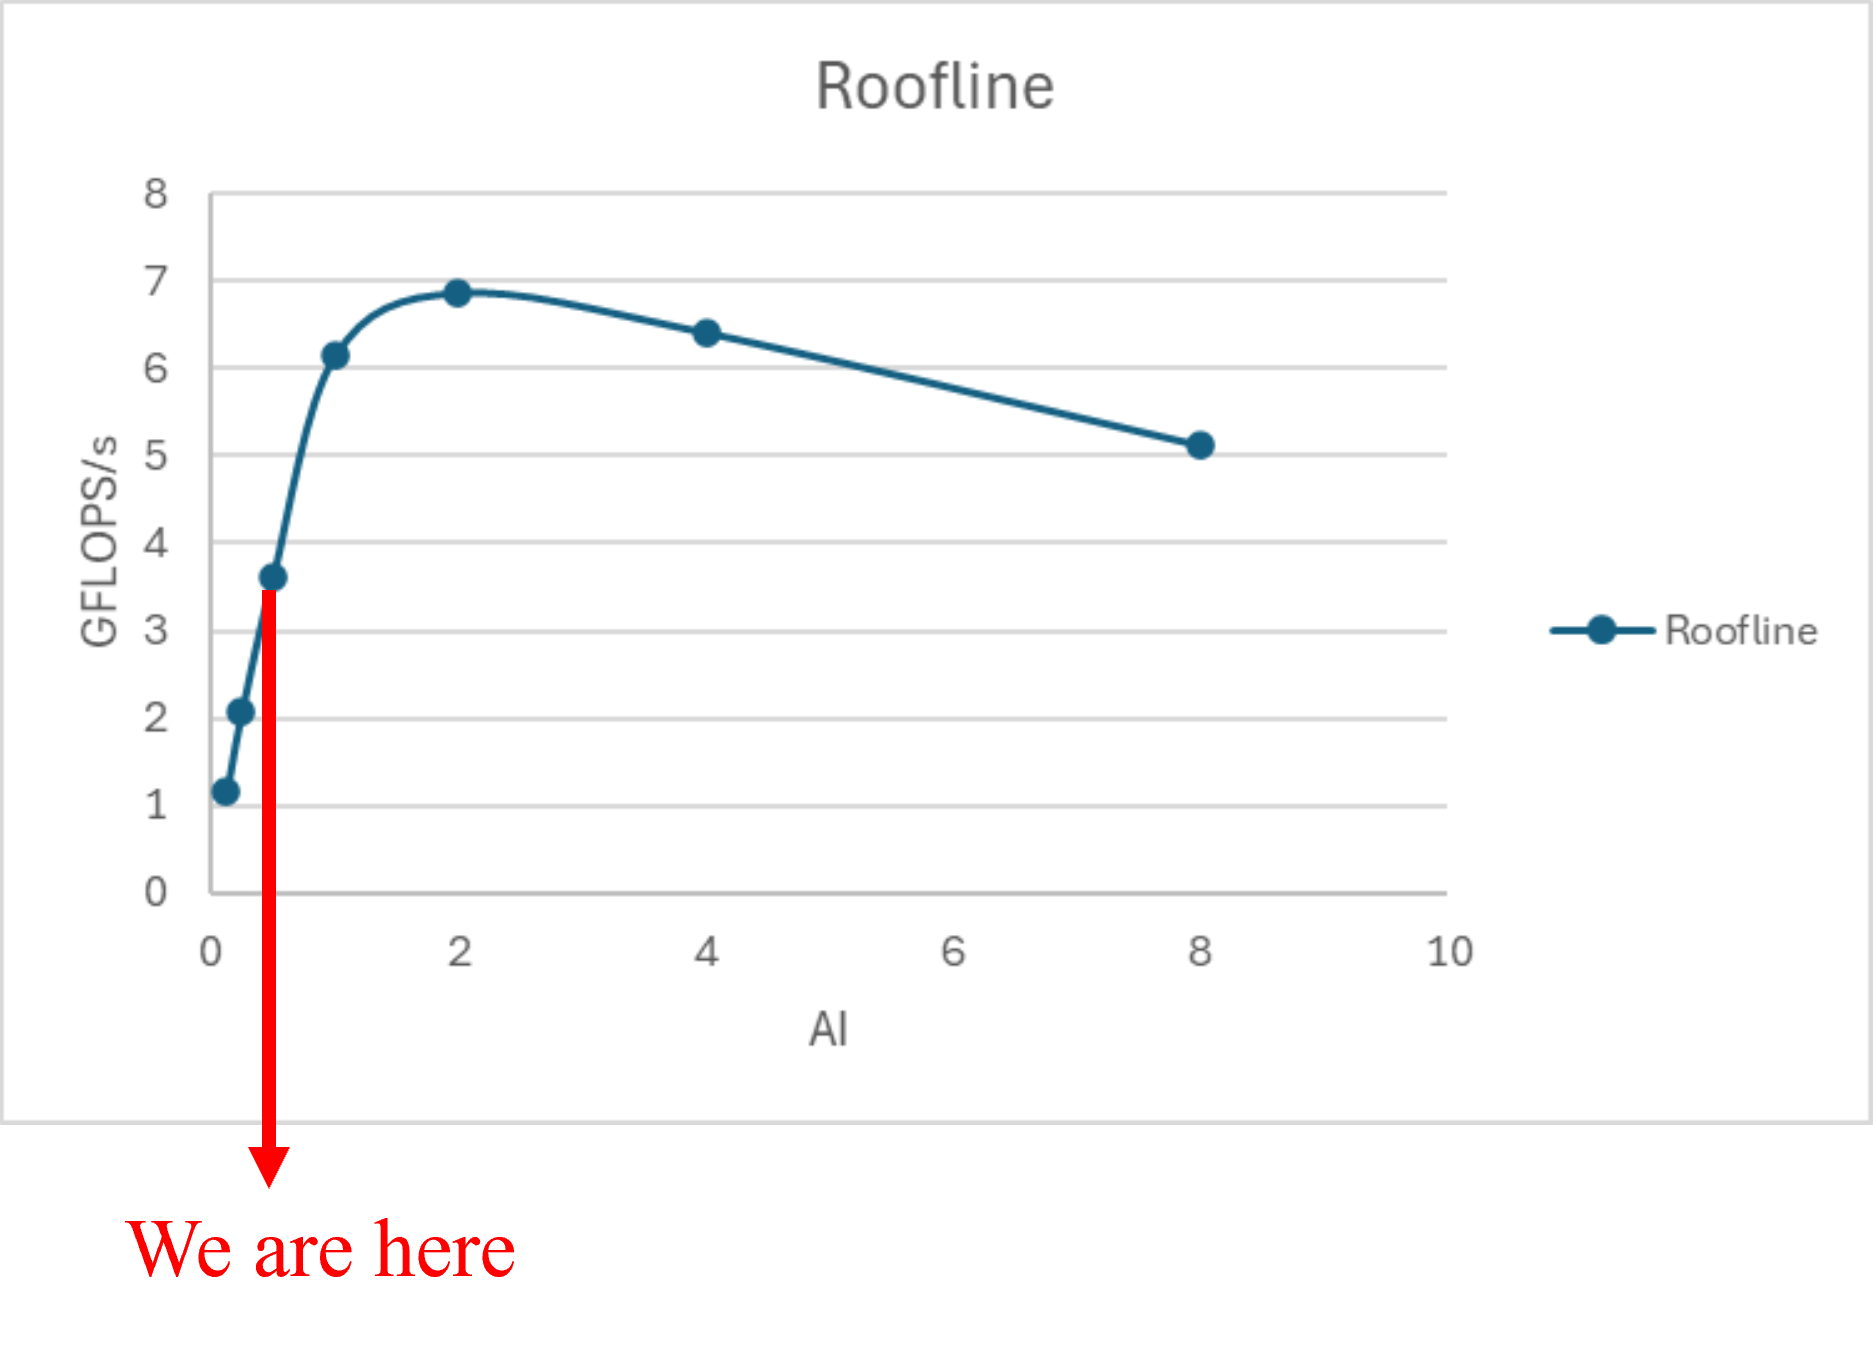
\includegraphics[width=0.65\linewidth]{roofline2.png}
\caption{Roofline-style throughput curve. AI $\approx$ 0.5--0.75
puts the stencil where the red arrow lands. On the bandwidth-bound
diagonal, well below the peak-compute plateau.}
\label{fig:roofline}
\end{figure}

\paragraph{Inner-loop micro-variants.} At $N{=}512$, 1 thread, 64
iters: \texttt{ij}-order gives CPE 0.39 with or without
\texttt{restrict}; \texttt{ji}-order jumps to 1.84 from cache
thrashing on stride-$N$ access. We keep \texttt{ij}-order.

\subsection{The full sweep}

Three forms in increasing order of complexity:

\begin{enumerate}[leftmargin=1.4em,itemsep=2pt,topsep=2pt]
  \item \textbf{Plain double-loop} (the \texttt{baseline} in every
        binary).
  \item \textbf{Spatially blocked.} Tile into $B{\times}B$ chunks
        (Figure~\ref{fig:spatial-blocking}). Helps once the working
        set exceeds L2.
  \item \textbf{Temporally blocked.} Shrinking trapezoid
        (Figure~\ref{fig:halo-time}); per-thread scratch is
        $2(B{+}2T)^2$ floats.
\end{enumerate}

\noindent At $B{=}128$, $T{=}8$ the work multiplier is
$(144/128)^2 \approx 1.27\times$. The bandwidth savings have to
outpace this overhead for temporal blocking to win.

\subsection{Loose ends}

\begin{itemize}[leftmargin=1.4em,itemsep=2pt,topsep=2pt]
  \item \textbf{Boundary copies.} Pass-through every sweep. Negligible
        vs interior data.
  \item \textbf{Per-tile scratch malloc.} The OMP version does
        \texttt{malloc(2*(B+2T)*(B+2T)*sizeof(float))} once per thread
        per super-step. At small $N$ this is real overhead
        (Figure~\ref{fig:size-sweep}, where temporal loses to baseline
        at $N{\leq}512$).
  \item \textbf{Convergence-norm reduction.} Used only in
        \texttt{sor2d\_rb.c} (one extra reduction per cell);
        responsible for slower per-iter timings in §\ref{sec:omega}.
  \item \textbf{Final swap.} A pointer swap, not memcpy.
\end{itemize}

\subsection{Stitching it together (real code)}

The actual temporal-blocking inner loop from \texttt{sor2d\_omp.c}
(stripped of declarations):

\begin{lstlisting}[language=C]
#pragma omp for collapse(2) schedule(static)
for (ti = 0; ti < ntiles_i; ti++) {
  for (tj = 0; tj < ntiles_j; tj++) {
    int i0 = 1 + ti*B,  j0 = 1 + tj*B;          /* tile origin in dst */
    int gi0 = i0 - T,   gj0 = j0 - T;           /* scratch origin     */

    /* (1) load (B+2T)x(B+2T) scratch from src */
    for (si = 0; si < S; si++)
      for (sj = 0; sj < S; sj++) {
        sa[si*S+sj] = src[clamp(gi0+si)*N + clamp(gj0+sj)];
      }
    memcpy(sb, sa, sizeof(float)*S*S);

    /* (2) T sub-steps on the in-scratch trapezoid */
    A = sa; Bp = sb;
    for (t = 0; t < T; t++) {
      memcpy(Bp, A, sizeof(float)*S*S);
      for (si = 1+t; si < S-1-t; si++)
        for (sj = 1+t; sj < S-1-t; sj++) {
          float s  = A[si*S+sj];
          float nb = 0.25f*(A[(si-1)*S+sj] + A[(si+1)*S+sj]
                          + A[si*S+sj-1]   + A[si*S+sj+1]);
          Bp[si*S+sj] = s - OMEGA*(s - nb);
        }
      tmp = A; A = Bp; Bp = tmp;
    }

    /* (3) write central B x B back to dst */
    for (si = T; si < T+B; si++)
      memcpy(dst + (gi0+si)*N + (gj0+T),
             A   + si*S       + T,
             B*sizeof(float));
  }
}
\end{lstlisting}

\texttt{collapse(2)} flattens the tile work-list so OMP can
load-balance. The inner \texttt{memcpy(Bp, A, ...)} preserves the
stale-halo perimeter so the compute loop is branch-free and the
compiler vectorises it cleanly.

\subsection{Code and Results}
\label{sec:cpu-results}

\subsubsection{Discussion of CPE}

\paragraph{Size sweep.} Figure~\ref{fig:size-sweep} (E02) shows the
cache-hierarchy story.

\begin{figure}[h!]
\centering
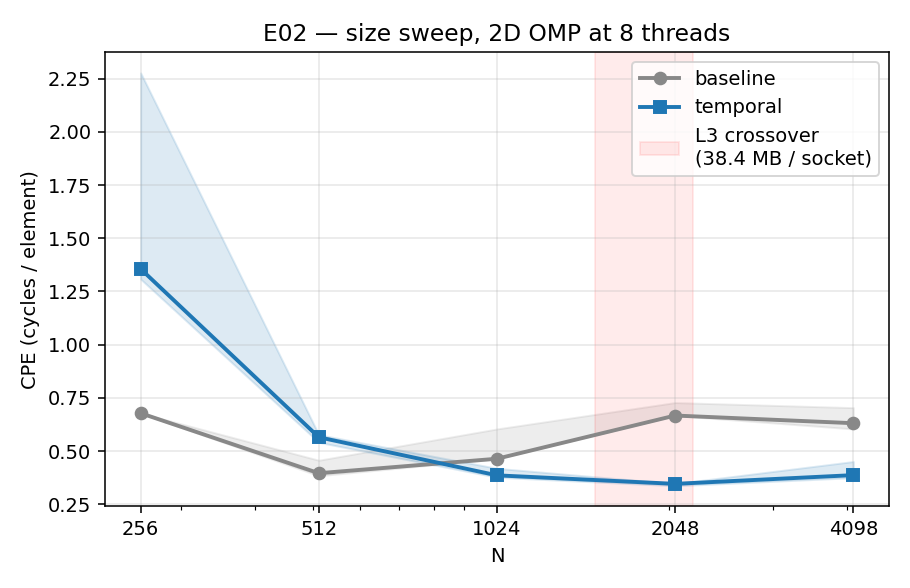
\includegraphics[width=0.62\linewidth]{e02_size_sweep.png}
\caption{2D OMP size sweep at 8 threads, $B{=}128$, $T{=}8$, iters=64.
The L3$\to$DRAM crossover lands between $N{=}1024$ and $N{=}2048$:
baseline CPE rises from 0.464 to 0.667 as the working set exceeds
38\,MB. Temporal stays at $\sim$0.35 across $N{=}1024$\,--$\,4098$
(L2-resident on its scratch) and wins 1.93$\times$ at $N{=}2048$.
Below L3 temporal loses: per-tile malloc + halo work cancel the
savings on a working set the baseline already had in cache.}
\label{fig:size-sweep}
\end{figure}

\noindent At $B{=}128$, $T{=}8$ the per-thread scratch is 81\,KB and
fits in L1 even at $N{=}4098$. The 2$\times$ ratio matches the
bandwidth ratio between cache and DRAM, give or take halo overhead.

\paragraph{Block size sweep.} At fixed $N{=}2048$ we sweep $B$
(Figure~\ref{fig:block-sweep}, E03).

\begin{figure}[h!]
\centering
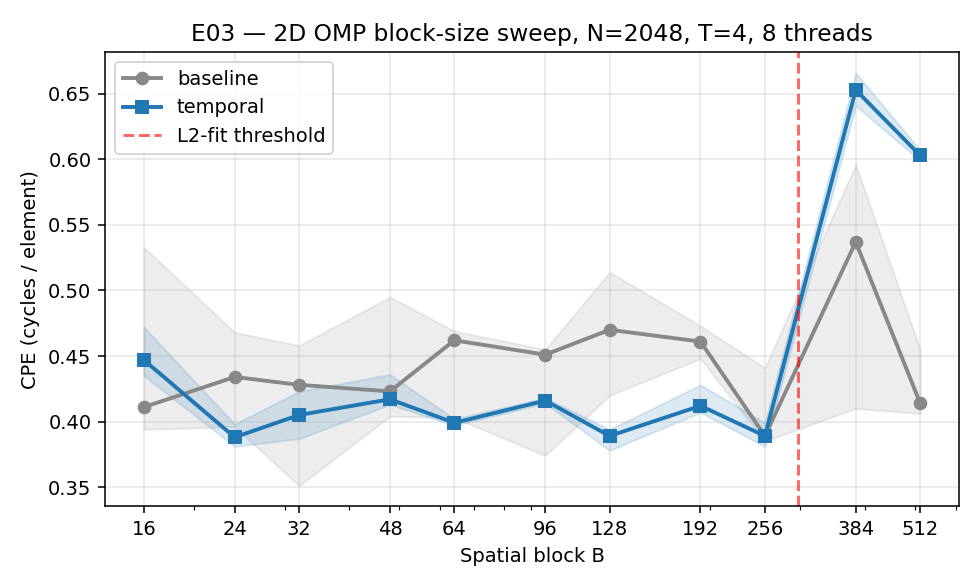
\includegraphics[width=0.62\linewidth]{e03_block_size.png}
\caption{Block-size sweep at $N{=}2048$, $T{=}4$, 8 threads.
Temporal has a wide plateau across $B{\in}[24, 256]$ at CPE
$\sim$0.39, then falls off a cliff at $B{\geq}384$. Red dashed line
is the L2-fit threshold ($B \leq 297$); beyond that, scratch spills
L2.}
\label{fig:block-sweep}
\end{figure}

\noindent We pick $B{=}128$: middle of the plateau, scratch fits L2,
and $2046/128 = 16$ tiles per axis aligns cleanly.

\paragraph{Halo / T sweep.} At fixed $B{=}128$ we sweep $T$
(Figure~\ref{fig:t-sweep}, E04).

\begin{figure}[h!]
\centering
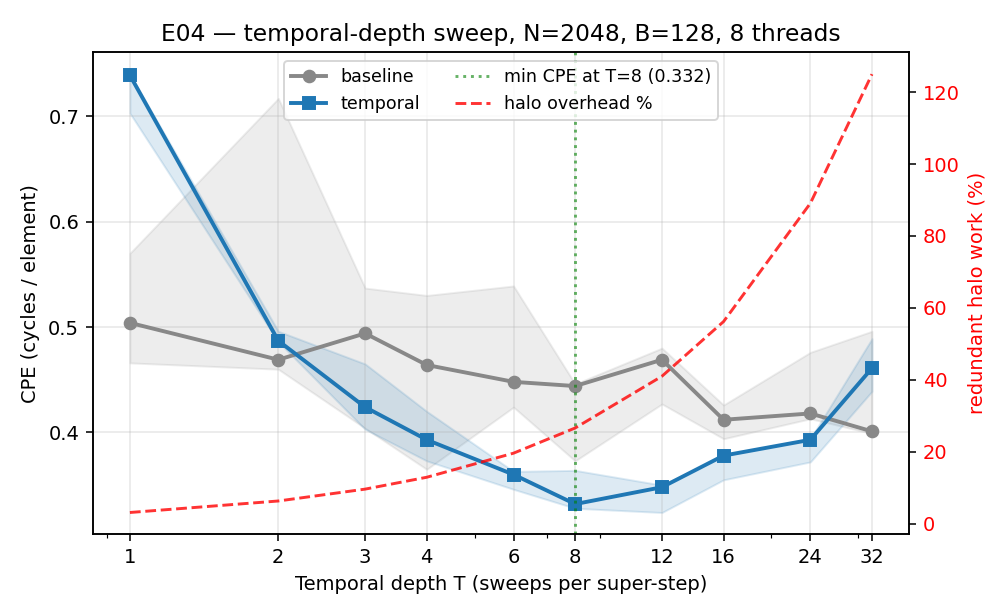
\includegraphics[width=0.65\linewidth]{e04_temporal_depth.png}
\caption{Temporal depth $T$ sweep at $N{=}2048$, $B{=}128$, 8
threads, iters=96. Left axis: CPE. Right axis: redundant halo work,
$((B{+}2T)^2/B^2 - 1){\cdot}100$. Optimum at $T{=}8$, CPE 0.332.}
\label{fig:t-sweep}
\end{figure}

\begin{table}[h!]
\centering
\renewcommand{\arraystretch}{1.1}
\begin{tabular}{rrrcr}
\toprule
$T$ & baseline CPE & temporal CPE & temp/base & halo overhead \\
\midrule
 1 & 0.504 & 0.739 & 1.47$\times$ &   3\% \\
 2 & 0.469 & 0.487 & 1.04$\times$ &   6\% \\
 4 & 0.464 & 0.393 & 0.85$\times$ &  13\% \\
 6 & 0.448 & 0.360 & 0.80$\times$ &  20\% \\
 8 & 0.444 & \textbf{0.332} & \textbf{0.75$\times$} & 27\% \\
12 & 0.469 & 0.348 & 0.74$\times$ &  41\% \\
16 & 0.412 & 0.378 & 0.92$\times$ &  56\% \\
24 & 0.418 & 0.393 & 0.94$\times$ &  89\% \\
32 & 0.401 & 0.461 & 1.15$\times$ & 125\% \\
\bottomrule
\end{tabular}
\caption{Halo/$T$ sweep. Best at $T{=}8$ (25\% faster than baseline);
$T{=}1$ pays scratch overhead with no DRAM-reuse benefit; $T{=}32$ is
swallowed by halo overhead.}
\label{tab:t-sweep}
\end{table}

\paragraph{Strong scaling and decomposition.}
Figure~\ref{fig:strong-scaling} shows strong scaling: temporal hits
91\% of perfect at 8 threads (7.31$\times$); baseline only 56\%
(4.49$\times$). At 1 thread temporal barely beats baseline
(1.08$\times$). Temporal blocking earns its keep only once
parallelism stresses DRAM.

\begin{figure}[h!]
\centering
\begin{subfigure}[b]{0.49\linewidth}
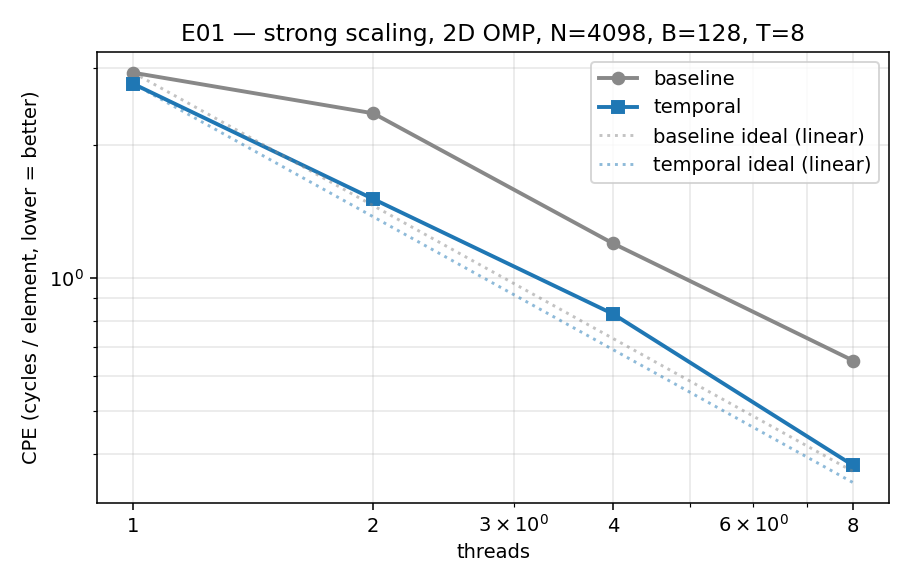
\includegraphics[width=\linewidth]{e01_strong_scaling.png}
\caption{Strong scaling (E01).}
\end{subfigure}\hfill
\begin{subfigure}[b]{0.49\linewidth}
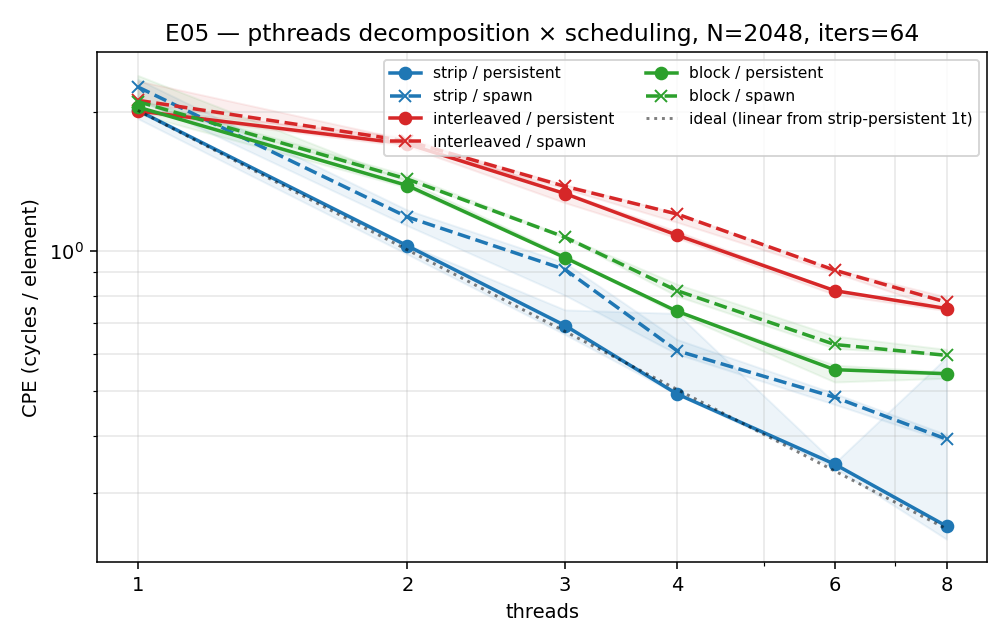
\includegraphics[width=\linewidth]{e05_decomposition.png}
\caption{Pthreads decomposition $\times$ schedule (E05).}
\end{subfigure}
\caption{Left: strong scaling at $N{=}4098$, $B{=}128$, $T{=}8$.
Right: 3 modes (strip / interleaved / 2D-block) $\times$ 2 schedules
(persistent / spawn). Strip-persistent at 8 threads: CPE 0.255,
7.89$\times$ scaling. Interleaved bottoms out at 2.67$\times$ from
false sharing on adjacent rows.}
\label{fig:strong-scaling}
\label{fig:decomp}
\end{figure}

Strip-persistent wins; interleaved loses to false sharing; 2D-block
sits in the middle. The \texttt{spawn}-vs-\texttt{persistent} gap is
largest for strip (1.54$\times$ slowdown) because strip's per-sweep
work is smallest.

\paragraph{Pthread spawn-overhead.} Figure~\ref{fig:spawn} (E07) is
the direct Lab-6-Part-1b answer.

\begin{figure}[h!]
\centering
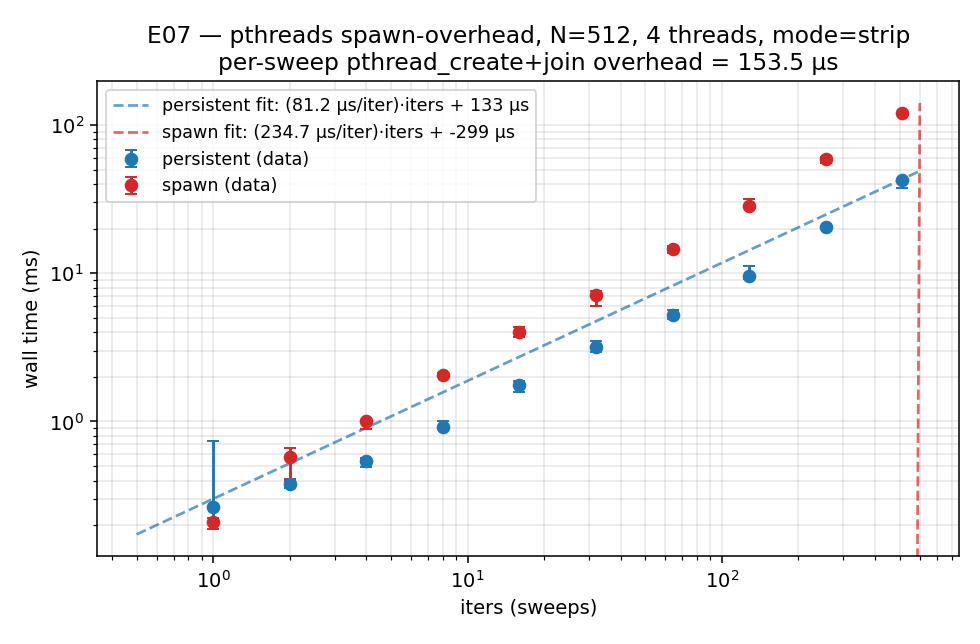
\includegraphics[width=0.62\linewidth]{e07_spawn_overhead.png}
\caption{Wall-time vs iters at $N{=}512$, 4 threads, mode=strip.
Persistent slope: 81\,$\mu$s/sweep (compute work). Spawn slope:
235\,$\mu$s/sweep. Slope difference 153\,$\mu$s is the per-sweep
\texttt{pthread\_create}+\texttt{join} overhead, larger than the
compute work itself.}
\label{fig:spawn}
\end{figure}

\noindent The per-sweep \texttt{pthread\_create} cost is roughly
153\,$\mu$s at 4 threads, or about 38\,$\mu$s per
\texttt{pthread\_create}+\texttt{join} pair. Spawning per sweep is a
1.89$\times$ tax on the kernel. This is why OpenMP under the hood
uses a persistent thread pool.

\paragraph{The OMP-vs-pthreads surprise.} OMP-8t baseline measured
CPE 0.667 at $N{=}2050$, while pthreads-strip-persistent at the same
$N$ measured $\sim$0.4. Pthreads beat OpenMP on the baseline sweep on
this machine. Likely a NUMA / first-touch interaction across the two
sockets; we didn't chase it further.

\subsubsection{Discussion of Iteration Number and Error}
\label{sec:omega}

The previous section was per-iter throughput. This one is iters-to-
tolerance, the algorithmic story.

\begin{figure}[h!]
\centering
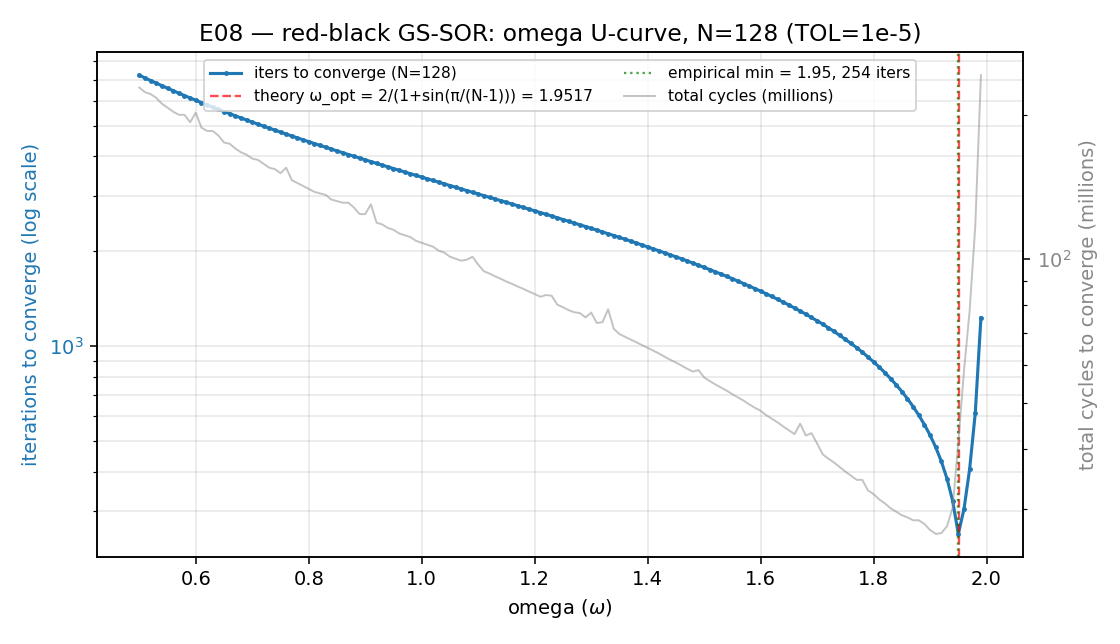
\includegraphics[width=0.7\linewidth]{e08_omega_ucurve.png}
\caption{Red-black GS-SOR omega U-curve at $N{=}128$, TOL=$10^{-5}$.
Theory $\omega_{\text{opt}} = 1.9517$ (red dashed) matches empirical
minimum at $\omega = 1.95$ (green dotted) to 0.1\%. 254 iters at
$\omega_{\text{opt}}$ vs 3{,}434 at $\omega{=}1$ (Gauss-Seidel) is a
13.5$\times$ fewer-iteration win.}
\label{fig:omega-ucurve}
\end{figure}

\noindent The cliff at $\omega > \omega_{\text{opt}}$ is sharp:
$\omega{=}1.99$ already gives back most of the win (1{,}230 iters).
Above $\omega{=}2$ the iteration is unconditionally divergent.

This is the project's biggest single algorithmic optimisation, and
the temporal-blocking kernels can't directly exploit it: damped
Jacobi at $\omega = 0.9$ lives on the under-relaxation side of the
curve; $\omega{>}1$ in the ping-pong form has spectral radius $>1$ on
large grids and diverges. The natural follow-up is a
temporal-blocking variant of red-black GS-SOR, which is the headline
future-work item.

\paragraph{FP32 round-off.} At $N{=}128$ and 254 iters the forward
error stays around $10^{-6}$, comfortably below TOL. At larger $N$ or
tighter TOL we'd need Kahan compensation or FP64.

\subsection{Overall comments}

\begin{enumerate}[leftmargin=1.4em,itemsep=2pt,topsep=2pt]
  \item \textbf{Temporal blocking only earns its keep in the
        bandwidth-bound regime.} Single-thread CPU was a wash
        (1.08$\times$); 8-thread + DRAM-spilling working set was
        2$\times$.
  \item \textbf{The $T$-sweet-spot is sharp.} $T{=}8$ wins by 25\%;
        $T{=}1$ loses to scratch overhead; $T{=}32$ loses to halo
        work.
  \item \textbf{Strip wins for 2D pthreads}, with 7.89$\times$
        scaling at 8 threads.
  \item \textbf{OMP can be slower than pthreads at the baseline
        sweep on a NUMA box.} Suspect: first-touch + cross-socket
        threads.
  \item \textbf{$\omega_{\text{opt}}$ is real and matters more than
        any per-iter optimisation we tried on CPU.} 13.5$\times$
        fewer iters at $N{=}128$.
\end{enumerate}

% =====================================================================
\section{To the GPU!}
\label{sec:gpu}
% =====================================================================

The L40S has $\sim$30$\times$ more memory bandwidth than one Xeon
socket (864 vs $\sim$280\,GB/s) and far more parallelism. The
question is whether temporal blocking's relative advantage shrinks on
the GPU. Spoiler: yes, it does.

\subsection{Memory allocation and transfer}

\begin{table}[h!]
\centering
\renewcommand{\arraystretch}{1.1}
\begin{tabular}{lrrr}
\toprule
\textbf{buffer} & \textbf{size} & \textbf{at $N{=}2048$} & \textbf{H$\to$D once?} \\
\midrule
\texttt{d\_src}                 & $N^2 \cdot 4$\,B   & 16\,MB & yes (init) \\
\texttt{d\_dst}                 & $N^2 \cdot 4$\,B   & 16\,MB & no (alloc only) \\
shared-mem scratch (per block)  & $2\cdot\textsc{tile}^2 \cdot 4$\,B & 8\,KB & no (per kernel) \\
constants                       & negligible    &        & yes \\
\bottomrule
\end{tabular}
\caption{GPU memory layout at $N{=}2048$, FP32. The dominant transfer
cost is the initial 16\,MB H$\to$D copy of \texttt{d\_src} ($\sim$0.6\,ms
at PCIe Gen4); after that, the iteration loop is fully on-device.}
\label{tab:gpu-mem}
\end{table}

We don't run a residual reduction inside the temporal kernel, so the
binary uses fixed iters rather than TOL-based stop. A real solver
would need a separate per-super-step reduction kernel.

\subsection{The parallelised hot loop on the GPU}

\paragraph{Vocabulary.} CPU ``thread'' maps to a CUDA \emph{block}
(private shared memory, \texttt{\_\_syncthreads()}); the CPU
$B{\times}B$ tile maps to a CUDA \textsc{tile}; warps inside a block
are the SIMD-lane equivalent.

\begin{lstlisting}[language=C]
__global__ void sor_temporal(const float *d_old, float *d_new,
                              int N, float omega, int tile, int halo)
{
  extern __shared__ float sshared[];
  float *sa = sshared, *sb = sshared + tile*tile;

  /* (1) clamp-to-edge load into both ping-pong buffers */
  load_tile_with_halo(sa, sb, d_old);
  __syncthreads();

  /* (2) HALO sub-steps; valid region shrinks 1 per side per step */
  for (int t = 0; t < halo; t++) {
    if (in_trapezoid(t)) compute_5pt_into_other_buffer();
    else                 carry_through();
    __syncthreads();
  }

  /* (3) write central INTER x INTER cells back to d_new */
  if (in_central_region) d_new[...] = result_from_current_buffer;
}
\end{lstlisting}

The kernel uses dynamic shared memory so we can vary
\textsc{tile}/\textsc{halo} at runtime. At \textsc{tile}$=24$ each
block has 576 threads (18 warps), and the SM can fit two blocks at
once. Good for occupancy.

\paragraph{Tuning sweep.} Figure~\ref{fig:gpu-tile-halo} (E09) is the
(\textsc{tile}, \textsc{halo}) heatmap.

\begin{figure}[h!]
\centering
\begin{subfigure}[b]{0.49\linewidth}
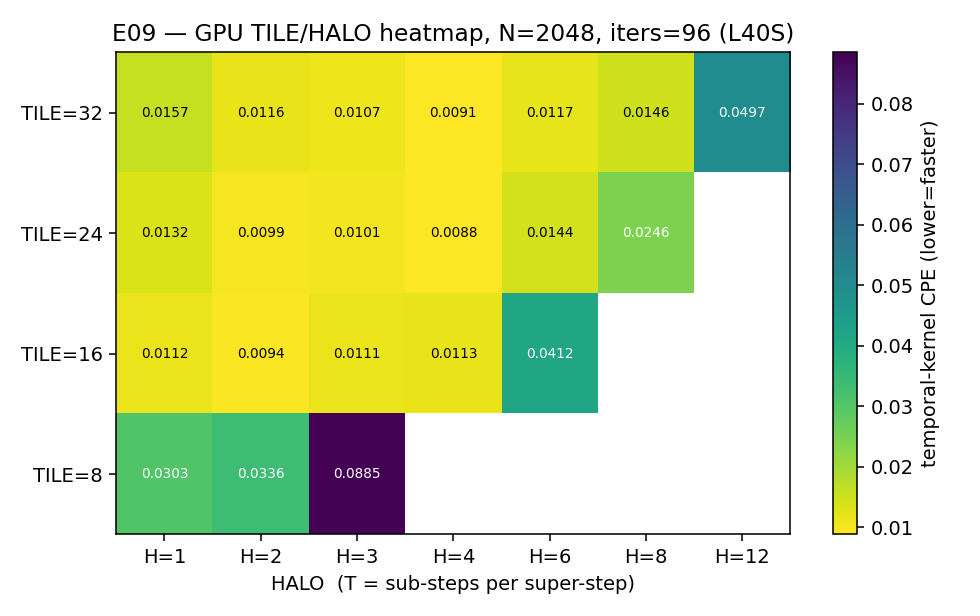
\includegraphics[width=\linewidth]{e09_tile_halo_heatmap.png}
\caption{Heatmap; dark = best CPE.}
\end{subfigure}\hfill
\begin{subfigure}[b]{0.49\linewidth}
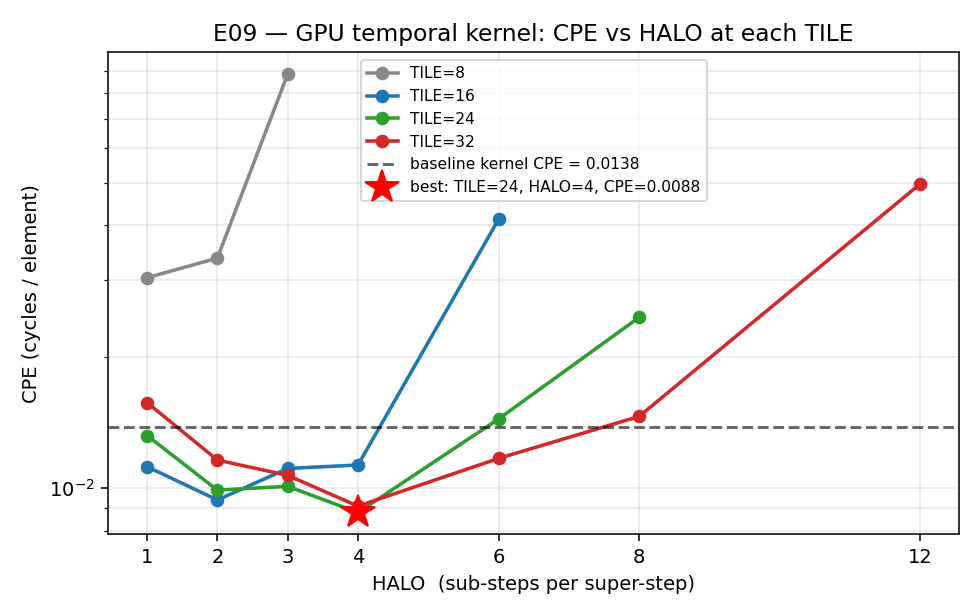
\includegraphics[width=\linewidth]{e09_tile_halo_lines.png}
\caption{CPE vs \textsc{halo}, one line per \textsc{tile}.}
\end{subfigure}
\caption{GPU 2D temporal sweep at $N{=}2048$, iters=96. Best at
$(\textsc{tile}{=}24,\, \textsc{halo}{=}4)$ with CPE 0.0088,
\textbf{1.56$\times$} over the per-launch baseline (CPE 0.0137).
Empirical rule: \textbf{HALO $\leq$ INTER/4}.}
\label{fig:gpu-tile-halo}
\end{figure}

\subsection{Partitioning the rest of the algorithm}

We had a real design choice between two GPU kernel structures:

\begin{enumerate}[leftmargin=1.4em,itemsep=2pt,topsep=2pt]
  \item \textbf{One kernel per stencil sub-step} (\texttt{sor\_sweep}).
        Easy to add a residual reduction between launches; pays
        $N^2 \cdot \text{iters}$ DRAM round-trips and one
        $\sim$30\,$\mu$s launch each time.
  \item \textbf{One temporal-blocked kernel} (\texttt{sor\_temporal}).
        Holds a $(\textsc{tile})^2$ shared-memory tile and does
        \textsc{halo} sub-steps per launch. Fewer DRAM trips and fewer
        launches, but mid-super-step residual checks are awkward.
\end{enumerate}

\noindent Both run side-by-side in the same binary. Shared memory at
TILE=24/HALO=4 is $2{\cdot}24^2{\cdot}4 = 4.5$\,KB per block, well
under the 100\,KB cap.

\subsection{Running it end-to-end}

\begin{figure}[h!]
\centering
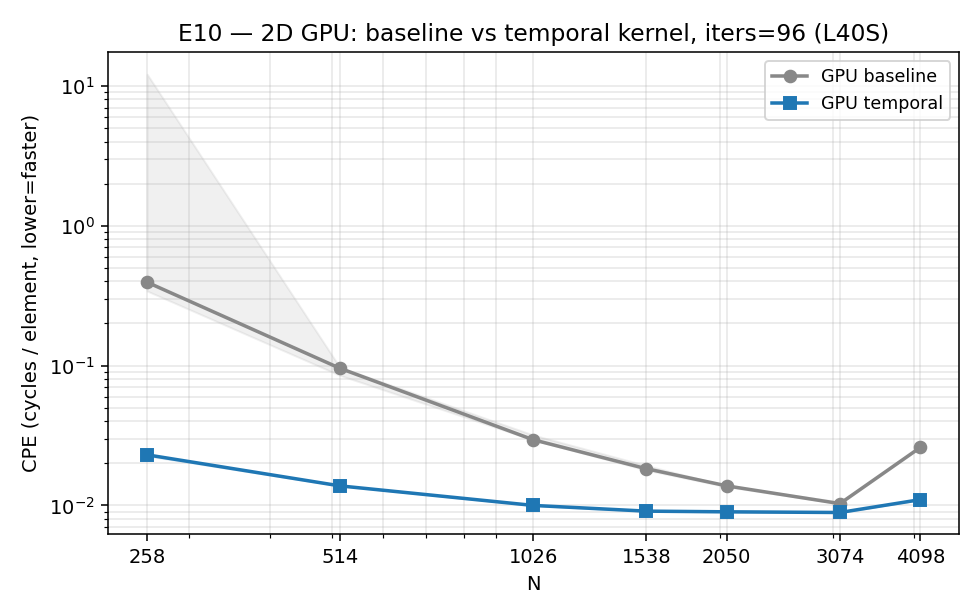
\includegraphics[width=0.7\linewidth]{e10_gpu_2d.png}
\caption{2D GPU baseline vs temporal across $N$, iters=96, defaults
TILE=32, HALO=4. At small $N$ the baseline is launch-overhead-
dominated; at $N{\geq}1024$ the steady-state speedup is a more honest
\textbf{1.5--3$\times$}. At $N{=}4098$ both kernels degrade (working
set $128$\,MB exceeds L40S's $\sim$96\,MB L2). Best 2D GPU CPE =
\textbf{0.0089} at $N{=}3074$.}
\label{fig:gpu-n}
\end{figure}

\begin{table}[h!]
\centering
\renewcommand{\arraystretch}{1.1}
\begin{tabular}{rrrrr}
\toprule
$N$ & baseline ms & temporal ms & baseline CPE & temporal CPE \\
\midrule
 258  &   2.7 & 0.16 & 0.395 & 0.023 \\
 514  &   1.8 & 0.27 & 0.096 & 0.014 \\
1026  &   2.4 & 0.83 & 0.030 & 0.010 \\
1538  &   3.7 & 1.86 & 0.018 & 0.0091 \\
2050  &   5.7 & 3.83 & 0.014 & 0.0090 \\
3074  &   9.5 & 8.18 & 0.010 & \textbf{0.0089} \\
4098  &  43.6 & 18.4 & 0.026 & 0.011 \\
\bottomrule
\end{tabular}
\caption{2D GPU N-sweep, iters=96. CPE values reported at CPNS=2.0
(lab convention).}
\label{tab:gpu-n}
\end{table}

\subsection{Discussion of GPU results}

\paragraph{The temporal/baseline ratio is smaller on GPU.} On CPU we
got 1.93$\times$ at the sweet spot; on GPU only 1.56$\times$. The
L40S has a $\sim$96\,MB L2, which already fits our $2N^2$ buffer at
$N{=}2050$, so the baseline kernel is mostly cache-resident and
temporal blocking has little to recover. The genuine memory-saving
win re-opens at $N{=}4098$ (128\,MB working set exceeds L2), where
the ratio is 2.36$\times$.

\paragraph{Apples to apples.} Quoted speedup vs the serial-CPU
baseline is 310$\times$. That's the headline but it isn't the honest
within-tier number. Honest comparisons:

\begin{itemize}[leftmargin=1.4em,itemsep=2pt,topsep=2pt]
  \item GPU-temporal vs OMP-temporal: $0.332 / 0.009 \approx
        \mathbf{37\times}$. ``GPU is better than 8-core CPU.''
  \item GPU-temporal vs GPU-baseline: $\mathbf{1.56\times}$.
        ``Shared-memory temporal blocking helps.''
  \item GPU-baseline vs serial-CPU baseline: $\mathbf{186\times}$.
        ``L40S is much better than one Xeon thread.''
\end{itemize}

\noindent The 310$\times$ is the product $186 \cdot 1.56$, presented
on its own it overstates the within-architecture optimisation.

\paragraph{The 3D GPU honest negative.} The 3D temporal kernel
(\texttt{sor3d\_gpu.cu}, TILE=8, HALO=2) loses to the 3D baseline at
$N \geq 194$. The 3D halo overhead is $7\times$ redundant work at
this configuration, much worse than the 2D case. The standard fix
(2.5D streaming) is on the future-work list.

\begin{figure}[h!]
\centering
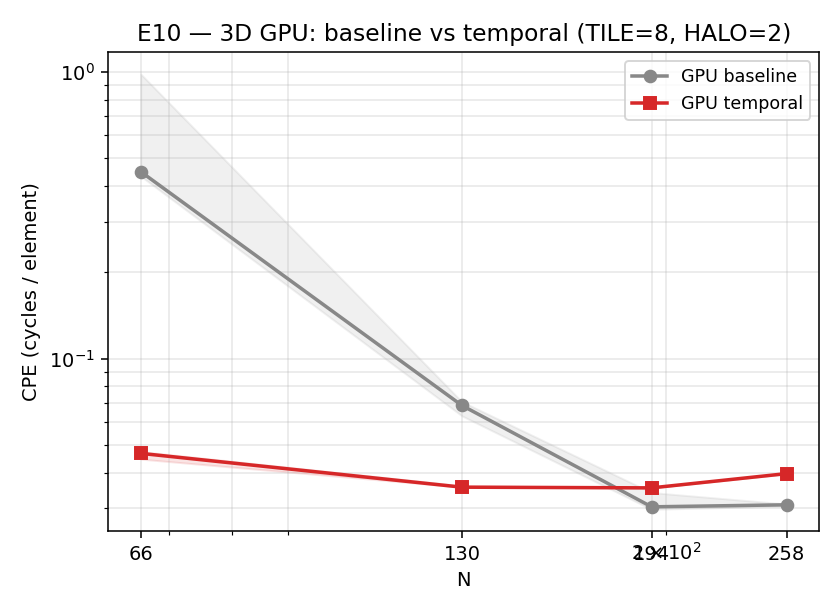
\includegraphics[width=0.55\linewidth]{e10_gpu_3d.png}
\caption{3D GPU baseline (grey) vs temporal (red) across $N$. At
$N{\geq}194$ the 3D halo overhead ($7\times$ redundant work) eats the
DRAM savings.}
\label{fig:gpu-3d}
\end{figure}

\paragraph{Cross-tier headline (E11).} At $N{=}2050$, iters=96, 8
threads:

\begin{table}[h!]
\centering
\renewcommand{\arraystretch}{1.1}
\begin{tabular}{lrr}
\toprule
\textbf{tier / kind} & \textbf{CPE} & \textbf{vs serial baseline} \\
\midrule
serial-CPU baseline           & 2.792    & 1.00$\times$ \\
serial-CPU temporal           & 2.586    & 1.08$\times$ \\
pthreads-8t-strip persistent  & 0.399    & 7.0$\times$ \\
OMP-8t baseline               & 0.667    & 4.2$\times$ \\
OMP-8t temporal               & 0.332    & 8.7$\times$ \\
GPU baseline                  & 0.015    & 186$\times$ \\
\textbf{GPU temporal}         & \textbf{0.009} & \textbf{310$\times$} \\
\bottomrule
\end{tabular}
\caption{Cross-tier CPE summary (E11).}
\label{tab:headline}
\end{table}

\noindent At CPNS=2.0, GPU temporal's 0.009 CPE corresponds to about
4.5\,ps per element. There's no easy 2$\times$ left without changing
the algorithm.

% =====================================================================
\section{Closing Thoughts}
\label{sec:closing}
% =====================================================================

\paragraph{What worked.} Temporal blocking on the bandwidth-bound CPU
regime was textbook: 1.93$\times$ at $N{=}2048$. Every CPU config was
bit-identical to its baseline. GPU shared-memory tiling was clean:
1.56$\times$ over the per-launch baseline at the right (TILE, HALO)
sweet spot.

\paragraph{What didn't.} Three things in increasing severity:

\begin{enumerate}[leftmargin=1.4em,itemsep=2pt,topsep=2pt]
  \item \textbf{Single-thread CPU temporal was a wash} (1.08$\times$).
        Per-tile malloc + halo work cancelled the bandwidth savings on
        a core where DRAM was already lightly loaded. Not a flaw, but
        worth being upfront about.
  \item \textbf{OMP baseline (CPE 0.667) was worse than pthreads
        (CPE 0.399)} at $N{=}2050$, 8 threads. Best guess: first-touch
        NUMA + cross-socket spreading. Honest unanswered.
  \item \textbf{3D GPU temporal lost to baseline at $N{\geq}194$.}
        Cubic tile $\Rightarrow$ surface-to-volume gets worse
        cubically; with TILE=8/HALO=2 the work multiplier is
        7$\times$. The fix (2.5D streaming) didn't make the cut.
\end{enumerate}

\paragraph{Precision.} (1) Lab-7's $\omega{=}1.85$ in
damped-Jacobi-ping-pong diverges on large grids; fixed by switching
to $\omega{=}0.9$ and flagging non-finite values explicitly. (2) FP32
round-off stays under TOL at every config we ran. (3) The
$N$-dependence of $\omega_{\text{opt}}$ in §\ref{sec:omega} matches
\eqref{eq:omega-opt}.

\paragraph{Future directions.}

\begin{enumerate}[leftmargin=1.4em,itemsep=2pt,topsep=2pt]
  \item \textbf{Red-black GS-SOR temporal kernel.} Combine the
        13.5$\times$ algorithmic win with the 1.56$\times$ per-iter
        win. Re-derive the trapezoid for paired half-sweeps. Expected
        $\sim$30$\times$ over the current GPU temporal.
  \item \textbf{2.5D-streaming for 3D GPU temporal} (Micikevicius
        2009). Slide a 3-z-plane window through shared memory; turns
        3D's $7\times$ halo into 2D's $0.78\times$.
  \item \textbf{Multigrid V-cycle.} The proper way to amplify SOR's
        per-iter speedup with a 5--20$\times$ fewer-iterations win on
        top.
  \item \textit{(Easter egg) Mixed precision.} FP64 residual
        accumulator with FP16/BF16 inner stencil; iterative-refinement
        style. Framework left commented out in the source.
\end{enumerate}

% =====================================================================
\section{Compilation instructions}
% =====================================================================

\begin{lstlisting}[language=bash]
# CPU binaries
gcc -O1 -std=gnu11 -fopenmp src/sor2d_omp.c -o build/sor2d_omp -lrt -lm
gcc -O1 -std=gnu11 -pthread src/sor2d_pth_decomp.c -o build/sor2d_pth_decomp \
                                                  -lpthread -lrt -lm

# GPU binaries
module load cuda/12.8
nvcc -O2 src/sor2d_gpu.cu -o build/sor2d_gpu
nvcc -O2 src/sor3d_gpu.cu -o build/sor3d_gpu

# Or just `make && make gpu`.
\end{lstlisting}

\noindent \texttt{-O1} matches the EC527 lab convention (keeps gcc
from auto-vectorising and complicating CPE analysis). \texttt{-O3
-march=native} would roughly halve baseline CPE on this CPU; we
chose course-style consistency over peak performance.

Preprocessor knobs:
\begin{itemize}[leftmargin=1.4em,itemsep=1pt,topsep=1pt]
  \item \texttt{N}, \texttt{B}, \texttt{T}, \texttt{ITERS}.
        Set at runtime via \texttt{argv}.
  \item \texttt{OMEGA}. Default 0.9; set to $\omega_{\text{opt}}(N)$
        for \texttt{sor2d\_rb}.
  \item \texttt{TOL}. Convergence tolerance; default $10^{-5}$.
  \item GPU runtime: \texttt{--tile T} and \texttt{--halo H}.
\end{itemize}

% =====================================================================
\section*{List of files}
% =====================================================================

Source files in \texttt{src/}:

\begin{itemize}[leftmargin=1.4em,itemsep=1pt,topsep=1pt]
  \item \texttt{sor2d\_cpu.c}, \texttt{sor3d\_cpu.c}. Single-thread
        baseline + temporal kernels.
  \item \texttt{sor2d\_omp.c}, \texttt{sor3d\_omp.c}. OMP versions.
  \item \texttt{sor2d\_pth.c}, \texttt{sor2d\_pth\_temporal.c},
        \texttt{sor3d\_pth\_temporal.c}. Pthreads versions
        (strip + barrier-per-sweep).
  \item \texttt{sor2d\_pth\_decomp.c}. Pthreads decomposition study
        (Figure~\ref{fig:decomp}).
  \item \texttt{sor3d\_omp\_part.c}. 3D OMP partitioning study
        (slab/pencil/cube).
  \item \texttt{sor2d\_rb.c}. Red-black GS-SOR with $\omega$ sweep
        (§\ref{sec:omega}).
  \item \texttt{sor2d\_gpu.cu}, \texttt{sor3d\_gpu.cu}. GPU baseline
        + shared-memory temporal kernels.
\end{itemize}

\end{document}
